\documentclass[11pt]{article}
    \title{\textbf{OrthOpt: a parallel tetrahedral mesh orthogonality optimizer}}
    \author{Moie Rousseau}
    \date{}
    
    \addtolength{\topmargin}{-3cm}
    \addtolength{\textheight}{3cm}
    
\usepackage{amsmath}
\usepackage{graphicx}


\begin{document}

\maketitle
\thispagestyle{empty}

\section{Introduction}

Talk about the advantage of TPFA. PEBI grid

Voronoi grid, but not conformal. VoroCrust, Collon Merland paper of quasi conformal. 

Only tetrahedral and pyramidal elements and vertices belong to triangular face were optimized.

Boundary faces did not needed to be optimized (it lack a point to define the cell center vector)

DuMuX simulator %https://bib.irb.hr/datoteka/581499.conference_book.pdf#page=177

TPFA standard in reservoir simulation, less computational cost, NTPFA for non K orthogonal grid %https://ntnuopen.ntnu.no/ntnu-xmlui/bitstream/handle/11250/2572391/20040_FULLTEXT.pdf?sequence=1&isAllowed=y

PorePy, use TPFA, with example of tet meshes %https://sci-hub.tf/https://link.springer.com/article/10.1007/s10596-020-10002-5

Utilise TFPA but non tet mesh %https://sci-hub.tf/https://ieeexplore.ieee.org/abstract/document/7502293

TPFA for richards %https://link.springer.com/article/10.1134/S1995080218070053

PFLOTRAN!

Quelque infos ici %file:///home/moise/T%C3%A9l%C3%A9chargements/173309-PA.pdf

Can not handle anisotropy easily %https://www.sciencedirect.com/science/article/pii/S0021999112000447

OPM software use TPFA %https://opm-project.org/?page_id=19

about mpfa method %https://ui.adsabs.harvard.edu/abs/2017AGUFM.H31D1541L/abstract

reduction of correction in OpenFOAM

Don't

Again


\section{Objective function}

Intent is to minimize for each face the angle between the face normal and the vector connecting the two cells center sharing the considered face by moving the mesh vertices. Therefore, the following objective function was defined:
\begin{equation}
f = \sum_{f \in faces} E_f = \sum_{f \in faces} w_f \left( 1 - r_f^T \cdot n_f \right) ^n
\label{objective_function}
\end{equation}
With $E_f$ the individual face error, $r_f$ the unit vector in the direction connecting the two cell center sharing the considering face $f$ and $n_f$ the unit face normal. 
The dot product give the cosinus of the face normal - cell center vector angle which is maximal when both vector are aligned (i.e. the mesh orthogonal at this face). 
The $w_f$ is a user specified weighting factor which allowed give higher importance to some connections compared to other, and the $n$ exponent represents a penalization factor for give more or less weight to high error versus low error. 

\section{Derivative of the objective function}

\subsection{Derivation of the objective function}

The general formula of the derivative of individual face error $E_f$ according to a mesh vertice $P$ is given by:
\begin{equation}
\frac{dE_f}{dP} = - n\ w_f\ \left( 1 - r_f^T \cdot n_f \right)^{n-1} \left(n_f^T \cdot \frac{d r_f}{dP}\ +\ r_f^T \cdot \frac{d n_f}{dP}\right)
\label{general_derivative_expression}
\end{equation}

Derivative of cell center vector and face normal according to mesh vertices required the knowledge of of the configuration of the mesh near the considered faces. Four distinct cases were identified (see X):
\begin{enumerate}
  \item Face is a triangle shared by two tetrahedra (common case). 
  \item Face is a triangle shared by one tetrahedron and one pyramid.
  \item Face is a triangle shared by two pyramids.
  \item Face is a quad shared by two pyramids
\end{enumerate}

In each case, the problem was generalized as follow: let $A$, $B$, $C$ (and $D$) be the three (four) vertices of the considered triangular (quad) face. 
Let $I$ and $J$ be the center of the two cells sharing the considered face so that the vector $R_f=\|R_f\|\ r_f = \overrightarrow{IJ}$ and the face normal $n_f = \overrightarrow{AB} \cdot \overrightarrow{AC}$ point in the same direction (i.e. $r_f^T \cdot n_f \geq 0$).
Vertices $E$ and $F$ designed the last vertices of the tetrahedra (pyramid) of center $I$ and $J$ respectively (see X).
The general problem was therefore to find the derivative of face area $ABC(D)$, the normal vector $n_f$ and the cell center vector $r_f$ according to mesh vertice $P$ if $P$ is either $A$, $E$ or $F$ ($B$, $C$ and $D$ cases are recovered by simply reordering face vertices). 

\begin{figure}[h]
  \centering
  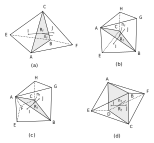
\includegraphics[width=\textwidth]{figures/cases.png}
  \label{cases_figure}
  \caption{The four different cases considered: (a) a triangular face shared by two tetrahedra, (b) shared by one tetrahedron and one pyramid, (c) share by two pyramids and (d) a quad face shared by two pyramids.}
\end{figure}

The general formula of the derivative of individual face error $E_f$ according to a mesh vertices $P$ could be therefore rewrite depending on the configuration considered and the position of $P$ in the given configuration (i.e. $P$ is $A$, $E$ or $F$):
\begin{equation}
\frac{dE_f}{dP} = \sum_{f\in\ conf(P=A)} \frac{dE_f}{dA} + \sum_{f\in\ conf(P=E)} \frac{dE_f}{dE} +
\sum_{f\in\ conf(P=F)} \frac{dE_f}{dF} 
\end{equation}



\subsection{General expressions of the unit vector derivatives}

\subsubsection{Unit cell center vector term}

Derivative of the unit cell center vector $r_f$ according to a point $P$ write (see Annexe):
\begin{equation}
\frac{d r_f}{dP}\ = 
- \frac{1}{\| R_f \|} \left[ \boldsymbol{I} - r_f \otimes r_f^T \right] \frac{d R_f}{dP}
\end{equation}
Also, the cell center vector derivative is either 0 for $P$ in position $A$, $\boldsymbol{I} /4$ if $P$ is in position $F$ or the opposite if in position $E$ (if non fixed). 
Therefore, the term implying the unit cell center vector in Eq. (\ref{general_derivative_expression}) write:
\begin{equation}
n_f^T\ \frac{d r_f}{dF}\ = - n_f^T\ \frac{d r_f}{dE} =
 \frac{1}{4 \| R_f \|} \left[n_f^T- n_f^T \cdot (r_f \otimes r_f^T) \right]
\end{equation}
Rearranging the parentesis finally lead to the general expression of the unit cell center vector derivative:
\begin{subequations}
\begin{align}
n_f^T\ \frac{d r_f}{dA}\ &=  0 \\
n_f^T\ \frac{d r_f}{dE}\ &= - \frac{1}{4 \| R_f \|} \left[ n_f^T - (n_f^T \cdot r_f)\ r_f^T \right] \\
n_f^T\ \frac{d r_f}{dF}\ &=  \frac{1}{4 \| R_f \|} \left[ n_f^T - (n_f^T \cdot r_f)\  r_f^T \right]
\end{align}
\end{subequations} 


\subsubsection{Unit face normal term}

Normal vector $N_f$ for the 4 cases could be computed using the cross product of vector $AB$ and $BC$:
\begin{equation}
N_f = (B-A) \times (C-B) = 
\begin{pmatrix}
(b_y-a_y)(c_z-b_z) - (c_y-b_y)(b_z-a_z)  \\
(b_z-a_z)(c_x-b_x) - (c_z-b_z)(b_x-a_x)  \\
(b_x-a_x)(c_y-b_y) - (c_x-b_x)(b_y-a_y) 
\end{pmatrix}
\end{equation}
The previous expression does not depend on other vertices than $A$, and thus only the derivative according to $A$ is non-null ($B$ and $C$ are recovered by renaming the vertice). Derivative according to $A$ writes:
\begin{equation}
\frac{d N_f}{dA}\ = \begin{pmatrix}
0 & (b_z-c_z) & (c_y-b_y) \\
(c_z-b_z) & 0 & (b_x-c_x) \\
(b_y-c_y) & (c_x-b_x) & 0
\end{pmatrix} 
\end{equation}
Therefore, the derivative of the term implying the unit normal $n_f$ is given by:
\begin{equation}
r_f^T\cdot \frac{d n_f}{dA}\ = 
 \frac{1}{\| N_f \|} \left[ r_f^T -  (r_f^T \cdot n_f)\ n_f^T \right] \frac{d N_f}{dA}
 \label{deriv_n_f}
\end{equation}

Computing the vector matrix product with the face normal and rearranging parentesis near the dyadic product product lead to the following simplified expression of Eq. (\ref{deriv_n_f}):
\begin{equation}
r_f^T\cdot \frac{d n_f}{dA}\ = 
 \frac{1}{\| N_f \|} \left[ \left[ r_f^T -  (r_f^T \cdot n_f)\ n_f^T \right]^T \times (C-B) \right]^T
\end{equation}


\subsection{Two dimensional case}

Polygonal



\section{Example application}

\subsection{Implementation}

A example implementation is proposed (REF) and uses the C++ programming language. 
This program takes as input the vertices coordinate in xyz format, the mesh element topology and the optimization parameters. 
Then, the mesh is decomposed and the internal connections are built. Optimization is carried using a on-purpose class call OrthOpt which compute the objective function and the derivative according to vertice position. 
Finally, optimization is carried using the L-BFGS algorithm of the L-BGFSpp library (REF). Stopping criteria include the maximum number of iteration, ..

The proposed implementation also benefits from the parallelization using OpenMP up to an arbitrary number of threads. 

\subsection{Mesh orthogonality optimization}

Examples applications include optimization of several meshes generated using popular 2D and 3D tetrahedral software such as TetGen, NETGEN and Gmsh.

Several meshes were generated with 
Compare with Gmsh, TetGen, Netgen


\subsection{Effect of penalization power}


\subsection{Application to numerical simulation}



\section{Discussion}

\subsection{Penalizing high error}
High orthogonality error could be more penalized by applying a power-law to individual face error. 

One may want to weigth the cost function with the face area in order to avor face orthogonality with high area. 
This weighting had also the advantage of possessing a less complicate derivative. 
However, meshes are often refined in sensitive place with low area faces, and therefore, this weigthing could be counter-productive in that case.

\section{Conclusion}

We hope you will enjoy using this release as much as we enjoyed creating it. If you have any further comments, suggestions or wish to report an issue, please visit \emph{\textbf{https://gummi.app}}. 




\section{Annexe}

\subsection{Expressions of cell center vectors and their derivative}

A general formula for the cell center vector write
\subsubsection{Case 1}

Center of a tetrahedra is given by the arithmetic mean of its four vertices:
\begin{subequations}
\begin{gather}
I = \frac{1}{4} (A + B + C + E) \\
J = \frac{1}{4} (A + B + C + F)
\end{gather}
\end{subequations} 
Therefore, cell center vector $R_f$ reads:
\begin{equation}
R_f = \| r_f \|\ r_f = J-I = \frac{1}{4} (F - E)
\end{equation}
Which permitted to express the derivative of $R_f$ according to a mesh vertice $P$ depending if $P$ is either $A$, $E$ or $F$:
\begin{subequations}
\begin{align}
\frac{d R_f}{d A} &= \ 0 \\
\frac{d R_f}{d F} &= - \frac{d R_f}{d E} = \frac{1}{4}\ \boldsymbol{I}
\end{align}
\end{subequations} 

\subsubsection{Case 2}

In the second case, the center of the tetrahedra $I$ and of the pyramid $J$ are given by:
\begin{subequations}
\begin{gather}
I = \frac{1}{4} (A + B + C + E) \\
J = \frac{A}{4} + \frac{1}{16} (B + C + G + H)
\end{gather}
\end{subequations} 
Therefore, cell center vector $R_f$ reads:
\begin{equation}
R_f = J-I = -\frac{E}{4} - \frac{3}{16} (B + C) + \frac{1}{16} ( G + H)
\end{equation}
In this case, only the $A$ and $E$ point are non fixed. Derivative of the cell center vector according to these two points is thus:
\begin{subequations}
\begin{align}
\frac{d R_f}{d A} &= \ 0 \\
\frac{d R_f}{d E} &= - \frac{1}{4}\ \boldsymbol{I}
\end{align}
\end{subequations}


\subsubsection{Case 3}

Center of both pyramids are given by:
\begin{subequations}
\begin{gather}
I = \frac{A}{4} + \frac{1}{16} (B + C + K + L) \\
J = \frac{A}{4} + \frac{1}{16} (B + C + G + H)
\end{gather}
\end{subequations} 
Cell center vector $R_f$ reads:
\begin{equation}
R_f = \frac{1}{16} ( G + H - K - L)
\end{equation}
In this case, only point $A$ is non fixed, which therefore give:
\begin{equation}
\frac{d R_f}{d A} = \ 0 
\end{equation}


\subsubsection{Case 4}

Center of both pyramids are given by:
\begin{subequations}
\begin{gather}
I = \frac{E}{4} + \frac{1}{16} (A + B + C + D) \\
J = \frac{F}{4} + \frac{1}{16} (A + B + C + D)
\end{gather}
\end{subequations} 
Cell center vector $R_f$ reads:
\begin{equation}
R_f = \frac{1}{4} (F-E)
\end{equation}
And derivative is:
\begin{equation}
\frac{d R_f}{d F} = - \frac{d R_f}{d E} = \frac{1}{4}\ \boldsymbol{I}
\end{equation}


\subsection{Expression of the normal vector and its derivative}

Thus, its derivative according to $A$ write:
\begin{equation}
\frac{dN_f}{dA} = 
\begin{pmatrix}
0 & (b_z-c_z) & (c_y-b_y) \\
(c_z-b_z) & 0 & (b_x-c_x) \\
(b_y-c_y) & (c_x-b_x) & 0
\end{pmatrix}
\end{equation}

\subsection{Expression of a unit vector derivative}
Starting from the definition of a unit vector $u$:
\begin{equation}
u = \frac{U}{N}
\end{equation}
With $U$ a non unit vector and $N$ its norm.
Derivate according to a particular point $X$ write:
\begin{equation}
\frac{du}{dX} = \frac{1}{N^2} \left[ N \frac{dU}{dX} - U \otimes \frac{dN}{dX} \right]
\end{equation}
Where the sign $\otimes$ represent the dyadic product. Derivative of the vector norm $N$ expresses:
\begin{equation}
\frac{dN}{dX} = \frac{d}{dX} \sqrt{\sum_i U_i^2} =
\frac{1}{N} \sum_i U_i \frac{dU_i}{dX}
\end{equation}
Which simplifies to:
\begin{equation}
\frac{dN}{dX} = \frac{1}{N}\ U^T \frac{dU}{dX}
\end{equation}
Replacing the above expression in those of the derivative of the unit vector $u$ leads, after dyatic product rearangement and factorization:
\begin{equation}
\frac{du}{dX} = \frac{1}{N} \left[ \boldsymbol{I} - u \otimes u^T \right] \frac{dU}{dX} = \frac{1}{N} \left[ \boldsymbol{I} - \frac{1}{N^2}\ U \otimes U^T \right] \frac{dU}{dX}
\end{equation}
With $\boldsymbol{I}$ the unit 3x3 diagonal matrix.




\end{document}

